\documentclass[a4paper, 11pt]{article}
\usepackage{comment} % enables the use of multi-line comments (\ifx \fi) 
\usepackage{lipsum} %This package just generates Lorem Ipsum filler text. 
\usepackage{fullpage} % changes the margin
\usepackage{amsmath}
\usepackage{graphicx}
\usepackage{multicol}
\usepackage{amssymb}
\usepackage{url}
%\usepackage{parskip}

%\setlength{\parindent}{0em}
%\setlength{\parskip}{1em}
%%\setlength{\baselineskip}{1.5em}
%\titlespacing\section{0pt}{11pt }{-3pt}
%\titlespacing\subsection{0pt}{10pt}{-3pt}
%\titlespacing\subsubsection{0pt}{10pt}{-3pt}


\begin{document}
\title{\textbf {
Machine Learning and Applications (MLAP)
Open Examination \linebreak
2016-2017}}
\date{}
\maketitle


\part*{The EM algorithm}
\section{Task 1}
%50 
For each state (square), the algorithm counts the number of times it was a starting state, the number of times it was transitioned to from each other state, and the number of times each reward was awarded in it. Counts are normalised so probabilities sum to 1.    

\section{Task 2}
%150
The implementation of the EM algorithm closely follows the steps outlined in Lecture 19. 


\begin{enumerate}


\item First the parameters are initialised with uniform distributions. The alpha recursion and the average log-likelihood for each episode are computed iteratively using the forward algorithm.
\begin{equation}
\alpha^n(h_t) = p(v_t^n|h_t)\sum\limits_{h_{t-1}}p(h_t|h_{t-1})\alpha^n(h_{t-1}) \qquad \qquad \alpha^n(h_1)=p(v_1^n|h_1)p(h_1)
\end{equation}

\begin{equation}
Log likelihood=\frac{1}{N} \sum\limits_{n=1}^N \sum\limits_{t=1}^T \log\sum\limits_{h_t} \alpha(h_t) 
\end{equation}

\item The beta recursion for each episode is computed iteratively using the backward algorithm.
\begin{equation}
\beta^n(h_{t-1})=\sum\limits_{h_t} p(v_t^n|h_t)p(h_t|h_{t-1}) \beta^n(h_t) \qquad \beta^n{h_T}=1
\end{equation}

\item When computing alpha and beta they are scaled in order to prevent numerical underflow \cite{Rabiner1989}.
\begin{equation}
\alpha^n(h_t)= \frac{\alpha^n(h_t)}{\sum\limits_{h_t}\alpha^n(h_t)} \qquad \beta^n(h_t) = \frac{\beta^n(h_t)}{\sum\limits_{h_t}\beta^n(h_t)}
\end{equation}

\item Hidden state marginals $\gamma$ and pairwise marginals $\xi$ are computed for each episode.
\begin{equation}
\gamma^n = p(h_t|v_{1:T}^n) = \frac{\alpha^n(h_t)\beta^n(h_t)}{\sum\limits_{h'_t} \alpha^n(h'_t)\beta^n(h'_t)}
\end{equation}
\begin{equation}
\xi^n = p(h_t,h_{t+1}|v^n_{1:T}) = \frac{
\alpha^n(h_t) p(v_{t+1}^n|h_{t+1}) p(h_{t+1}|h_t) \beta^n(h_{t+1})} 
{\sum\limits_{h'_t}\sum\limits_{h'_{t+1}}\alpha^n(h'_t) p(v_{t+1}^n|h'_{t+1}) p(h'_{t+1}|h'_t) \beta^n(h'_{t+1})}
\end{equation}

\item Initial, transition and emission probabilities are updated using hidden state marginals and pairwise marginals in three separate function. The parameter matrices are normalised in order for probabilities to sum to 1.
\begin{equation}
p^{new}(h_1) = \frac{1}{N}\sum\limits_{n=1}^N \gamma^n(h_1) 
\end{equation}
\begin{equation}
p^{new}(h_{t+1}|h_t) = \frac{\sum\limits_{n=1}^N \sum\limits_{t=1}^{T_n-1}\xi^n(h_t,h_{t+1})}
{ \sum\limits_{n=1}^N \sum\limits_{t=1}^{T_n-1} \sum\limits_{h_{t+1}} \xi^n(h_t,h_{t+1})}
\end{equation}
\begin{equation}
p^{new}(v_t=i|h_t) = \frac{\sum\limits_{n=1}^N \sum\limits_{t=1}^{T_n-1}  I[v_t^n = i] \gamma^n(h_t)}
{ \sum\limits_{n=1}^N \sum\limits_{t=1}^{T_n-1} \gamma^n(h_t)} 
\end{equation}



\item If the change in log-likelihood is smaller than the threshold 0.01, the algorithm terminates, otherwise it proceeds with the next iteration.
\end{enumerate}


\section{Task 3}
%200
\subsection{Difference in log-likelihood for different EM runs}
The EM algorithm is guaranteed to converge to a local maximum of the likelihood. This means that the closest local maximum to the initial position, in the search space, is reached at each run.  When parameters are initialised randomly, at each run the algorithm is likely to converge to a different local maximum, compared to previous runs, since the starting conditions are different.

\subsubsection{Uniform vs random initialisation}
When using uniform distributions for initial parameters of the EM algorithm, the transition and initial probabilities do not change. The EM algorithm ignores the fact that we have hidden variables and computes the maximum likelihood estimate of the reward, regardless of the state. This is because the priors for hidden variables are constant with respect to the posterior.
On the other hand random initialisation of the algorithm results in evolution of initial and transition probabilities, because we are defining non-constant priors with respect to the posterior.  

\section{Task 4}
%20
Transition probabilities are initialised to 0, for transitions from non neighbouring squares and squares with walls between them.


\pagebreak
\part*{Manifold learning}
\section{Algorithm Descriptions}
%10 marks 300 words

\subsection{Isomap}
%3.33 marks 100 words
Isomap \cite{Tenenbaum2000} aims to project a set of data points from the high dimensional space, in which they exist, to a lower dimensional representation, while preserving the global geodesic distances between them. The algorithm assumes data points are embedded in an intrinsically low dimensional manifold in the higher dimensional space. It starts by constructing a nearest neighbour graph of the data points, in which only data points which are close to each other are connected. Then it computes the euclidean distances between neighbouring data points. After that it computes the distances for all other data points by taking the shortest path between them in the graph. The computed distances are approximate geodesic distances in the manifold. In the last step the algorithm uses the MDS algorithm to find the lower dimensional representation of the data.

%estimating the geodesic distance between neighbouring data points. 
%It does this by first finding the aproximate geodesinc dinstances between data points on the manifold. Then uses MDS to project the data into the lower dimensional representation
%
%The algorithm starts by computing the nearest neighbour graph, which contains the euclidean distances between each data point and its closest neighbours. The closest neighbours are determined using either k nearest neighbour or $\epsilon$-neighbourhoods algorithm. Then, using a shortest path algorithm the distances between non-neighbouring points are computed. All the computted distances are aproximate geodesic distances of data points on a the low dimensional manifold. Then the MDS algorithm is applyed to the the matrix of distances and the first m eigenvectors (in order of their corresponding eigenvalues) obtained for each data point are the coordinates of the point in the lower dimensional space. 

\subsection{Laplacian Eigenmap}
%3.33 marks 100 words
Laplacian Eigenmap \cite{Belkin2003} also projects data to a lower dimensional representation. In contrast to Isomap, Laplacian Eigenmap aims to preserve only local distance information. In the first step of the algorithm, the nearest neighbour graph is computed as in Isomap, with edges between points which are close to each other. The distances between neighbouring points are either set to 1 or computed from the euclidean distances, using a heat kernel. The new coordinates for the data points are the eigenvector solutions (in order of their eigenvalues) to the generalised eigenvector problem for the graph Laplacian and diagonal weight matrices. The eigenvector with the smallest eigenvalue is excluded. 


\subsection{Locality Preserving Projection}
%3.33 marks 100 words
Locality Preserving Projection \cite{Xiaofei2005} follows the same steps as Laplacian Eigenmap - constructing a nearest neighbour graph and computing the edge weights(distances). The generalised eigenvector problem is solved for the Laplacian and diagonal weight matrices of the graph, each pre and post multiplied by the matrix of data vectors and matrix of data vectors transposed, respectively. The first $m$ rows of The resulting eigenvector matrix, multiplied by the a data vector, gives the new $m$-dimensional representation of the data vector. In contrast to Laplacian Eigenmap, this algorithm is linear and can be kernelised.


\section{Data proximity graph}
%5 marks 200 words
All three methods assume data lives on an intrinsically low dimensional manifold. In Isomap, a data proximity graph is used to approximate geodesic distances between each two data points on the manifold (global distances). In the other two approaches the graph is used to approximate distances only between points, that are close to each other (local distances). In Isomap the local distances in the graph are euclidean $d_{ij} = ||\vec{x}_i - \vec{x}_j||$. In the other two approaches a heat kernel is used for local distances $d_{ij} = \exp{\Big(-\frac{||\vec{x}_i - \vec{x}_j||^2}{t}	\Big)}$ or they are simply set to 1.



%In the other two approaches the weights in the proximity graph are either set to one or to an exponential of the euclidean distances between data points. The graph Laplacian matrix and diagonal weight matrix are directly used in the calculation of the lower dimensional projection of the data points. Here, the data proximity graph is used to model distances within data clusters, rather than the exact distances between each two data points.


\section{Laplacian matrix and Fiedler vector}
%5 marks 200 words
\subsection{Laplacian matrix construction} \label{sec:laplacian}
%2.5 100 words
A weighted graph $G(V,E)$ has vertices $v \in V$, edges between nodes $i$ and $j$ $e_{ij} \in V$ and weights of edges $w(e) \in \mathbb{R}$ (for an unweighted graph assume $w(e)=1$). The adjacency matrix of a graph $G(V,E)$ is a square matrix defined as:
\begin{equation}
  A_{ij} =
  \begin{cases}
    1 & \quad  \text{if } e_{ij} \in E \quad \text{ for } i, j \in V\\
    0  & \quad otherwise\\
  \end{cases}
\end{equation}

The degree matrix $D$ of a graph  is a diagonal matrix, which contains the degree(number of edges connected to) each node along the diagonal:
\begin{equation}
D_{ii} =
    \sum_j^N{A_{ij}} \quad \text{ for } \forall i, \forall j \in V
    \qquad \qquad
    D_{ij} = 0 \quad \text{ for } \forall i, \forall j \in V, \text{ where } i \neq j
\end{equation}

The weight matrix $W$ and diagonal weight matrix $D'$ of $G(V,E)$ are defined in the following two equations:
\begin{equation} \label{eq:weightmatrix}
  W_{ij} =
  \begin{cases}
    w(e_{ij}) & \quad \text{ if } e_{ij} \in E  \quad \text{ for } i \in V, j \in V\\
    0  & \quad otherwise\\
  \end{cases}
\end{equation} 
\begin{equation} \label{eq:diagweightmatrix}
D'_{ii} =
    \sum_j^N{W_{ij}} \quad \text{ for } \forall i, \forall j \in V
    \qquad \qquad
    D'_{ij} = 0 \quad \text{ for } \forall i, \forall j \in V, \text{ where } i \neq j
\end{equation}

The Laplacian matrix $L$ of a weighted graph is:
\begin{equation}
 L = D' - W  
\end{equation}

The Laplacian matrix $L$ of an unweighted graph 
\begin{equation}
L = D' - W = D - A
\end{equation}


A derviation of the Laplacian of the unweighted undirected graph in figure \ref{fig:graph} is shown in equation \ref{eq:laplacian}. The example was taken from \cite{wikipedia2017}.
\begin{figure}[h]
  \centering
    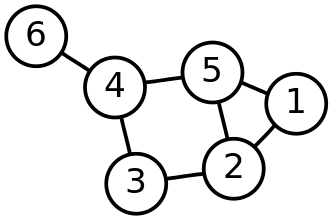
\includegraphics[width=0.2\textwidth]{figures/graph.png}
	\caption{Unweighted Graph}    
    \label{fig:graph}
\end{figure}

\begin{equation} \label{eq:laplacian}
A = 
 \begin{pmatrix}
  0 & 1 & 0 & 0 & 1 & 0 \\
  1 & 0 & 1 & 0 & 1 & 0 \\
  0 & 1 & 0 & 1 & 0 & 0 \\
  0 & 0 & 1 & 0 & 1 & 1 \\
  1 & 1 & 0 & 1 & 0 & 0 \\  
  0 & 0 & 0 & 1 & 0 & 0 \\
  \end{pmatrix}
D = 
 \begin{pmatrix}
  2 & 0 & 0 & 0 & 0 & 0 \\
  0 & 3 & 0 & 0 & 0 & 0 \\
  0 & 0 & 2 & 0 & 0 & 0 \\
  0 & 0 & 0 & 3 & 0 & 0 \\
  0 & 0 & 0 & 0 & 3 & 0 \\  
  0 & 0 & 0 & 0 & 0 & 1 \\
 \end{pmatrix} 
 \quad  
L = D - A = 
 \begin{pmatrix}
  2 & 0 & 0 & 0 & 0 & 0 \\
  0 & 3 & 0 & 0 & 0 & 0 \\
  0 & 0 & 2 & 0 & 0 & 0 \\
  0 & 0 & 0 & 3 & 0 & 0 \\
  0 & 0 & 0 & 0 & 3 & 0 \\  
  0 & 0 & 0 & 0 & 0 & 1 \\
  \end{pmatrix}
\end{equation}

\subsection{Significance of Fiedler vector} \label{sec:fiedler}
The second smallest eigenvalue of the Laplacian matrix of a graph is known as the algebraic connectivity of the graph \cite{Fiedler1973}. It is greater than zero iff the graph is connected. The eigenvector corresponding to the algebraic connectivity is known as the Fiedler vector \cite{Fiedler1975}.  Groups of values of the components of the Fiedler vector which are close to each other naturally represent clusters in the graph. This is why it has been used in various clustering and graph partition algorithms.


\section{Algorithm}
%15 marks 400 words
Given a set of data $X = \{\vec{x}_1, \dots \vec{x}_N\}$ where $\vec{x}_i$ is the $i$-th vector which is of length $d$ and there are $N$ such vectors, the three algorithms go through the following steps:

\subsection{Isomap} \label{sec:isomap}
%5 marks 125 words

\begin{enumerate}

\item Initialise nearest neighbour graph $G(V,E)$, with weight matrix $W$, with $V = \{1, \dots , N\}$ and $E = \emptyset$. 

\item Construct an edge between vertices $i$ and $j$ if $\vec{x}_i$ and $\vec{x}_j$ are "close" to each other, using one of the following methods: 

	\begin{multicols}{2}
	\begin{enumerate}
	\item 
	For each pair of nodes $i,j \in V$,  construct an 		edge between $i$ and $j$ iff $i$ is among the $k$ nearest 		neighbours of $j$ or $j$ is among the $k$ nearest 				neighbours of $i$, where $k$ is a user defined constant and $i \neq j$.  

	\columnbreak
	\item 
	For each pair of nodes $i,j \in V$,  construct an 		edge between $i$ and $j$ iff $||\vec{x}_i - \vec{x}_j|| < 	\epsilon$, where $\epsilon$ is a user defined constant and $i \neq j$.  

	\end{enumerate}
	\end{multicols}

\item Set weights of edges to euclidean distances.

	\begin{equation}
	W_{ij} = 
	\begin{cases}
	||\vec{x}_i - \vec{x}_j|| & \text{if } e_{ij} \in E \\
	0 & \text{otherwise}
	
	\end{cases}
	\end{equation}


	\item Initialise distance matrix $D$.
	\begin{equation}
	D_{ij} = 
	\begin{cases}
	W_{ij} & \text{if } e_{ij} \in E \\
	0 & \text{if } i = j	\\
	\infty & \text{otherwise}	
	\end{cases}
	\end{equation}

	\item Replace all distances in $D$ with their shortest 			paths in $G$.
	
	\begin{equation}
	D_{ij} = \min(D_{ij}, e_{ik} + e_{kj}) \quad \text{for } 		k=1,2,\dots N, \text{ where } e_{ik}, e_{kj} \in E
	\end{equation}


	\item Compute the squared distance matrix $S$.
	\begin{equation}
	S_{ij} = D_{ij}^2 \quad \text{for }\forall i \in [1;N], \forall j \in [1;N]
	\end{equation}

	\item Compute kernel matrix $K$ using equation \ref{eq:K}, 		where $I$ is the identity matrix and $J$ is the matrix of 		all	ones.	
	\begin{equation} \label{eq:K}
	K = \frac{(I-\frac{J}{N})S(I-\frac{J}{N})}{2}  
	\end{equation}

	\item Compute the eigenvalues and eigenvectors of $K$.
	\begin{equation}
	K = U \Lambda U^T
	\end{equation}	
	
	\item Assuming the resulting eigenvectors are $\vec{u}_1, \dots \vec{u}_N$, where  $\vec{u}_{l}(i)$ is the $i$-th component of the $l$-th vector, and the corresponding eigenvalues, ordered in decreasing order, are $\lambda_1 > \lambda_2 > \dots >\lambda_N$, the new $m$-dimensional representation of each vector $\vec{x}_i \in X$ is $\vec{y}_i$ and is given by:
	\begin{equation}
	\vec{y}_{i}(l) =\sqrt{\lambda_l} \vec{u}_{l}(i) \quad \text{ for } l = 1, \dots m, \text{ for } i = 1, \dots N \quad \text{ where } m<d
	\end{equation}	

\end{enumerate}

\subsection{Laplacian Eigenmap} \label{sec:eigenmap}
%5 marks 125 words
\begin{enumerate}
	\item Initialise nearest neighbour graph $G(V,E)$, with weight matrix $W$, with $V = \{1, \dots , N\}$ and $E = \emptyset$. 

	\item Construct an edge between vertices $i$ and $j$ if $\vec{x}_i$ and $\vec{x}_j$ are "close" to each other, using either k nearest neighbours or $\epsilon$-neighbourhoods algorithms described in step \ref{itm:knn}  and step \ref{itm:epsilon} 	of the Isomap algorithm (section \ref{sec:isomap}).
	
	\begin{multicols}{2}
	\begin{enumerate}
	\item \label{itm:knn} \textbf{K nearest neighbours} \\
	For each pair of nodes $i,j \in V$,  construct an 		edge between $i$ and $j$ iff $i$ is among the $k$ nearest 		neighbours of $j$ or $j$ is among the $k$ nearest 				neighbours of $i$, where $k$ is a user defined constant and $i \neq j$.  

	\columnbreak
	\item \label{itm:epsilon} \textbf{$\boldsymbol{\epsilon}$-neighbourhoods} \\
	For each pair of nodes $i,j \in V$,  construct an 		edge between $i$ and $j$ iff $||\vec{x}_i - \vec{x}_j||^2 < 	\epsilon$, where $\epsilon$ is a user defined constant and $i \neq j$.  

	\end{enumerate}
	\end{multicols}

	\item Set weights of the created edges using heat kernel or 	simple methods described below.

	\begin{multicols}{2}
	\begin{enumerate}
	\item \textbf{Heat kernel} \label{itm:heatkernel}
	\begin{equation}
	W_{ij} = \exp{\Big(-\frac{||\vec{x}_i - \vec{x}_j||^2}{t}		\Big)}
	\end{equation}	  
	$t$ is a user defined constant.

	\columnbreak
	\item \textbf{Simple} \label{itm:simple}
	\begin{equation}
		W_{ij} = 1
	\end{equation}

	\end{enumerate}
	\end{multicols}


	\item If the graph $G$ is not connected proceed with the next steps of the algorithm for each connected part of $G$. The number of connected disjoint parts of a graph correspond to the number of zero eigenvalues of the Laplacian matrix of the graph (see section \ref{sec:fiedler}).
	
	\item Compute the Laplacian matrix $L = D - W$ of the graph as described in section \ref{sec:laplacian}, using the weight matrix $W$ and the diagonal weight matrix $D$, where $D_{ii} = \sum_{j=1}^N W_{ji}$.


	\item Solve the generalised eigenvector problem for $L$ and 	$D$.
	\begin{equation} \label{eq:gen_eig1}
	L\Phi = \Lambda D \Phi
	\end{equation}
	
\item Assuming the resulting eigenvectors are $\vec{\phi}_0, \dots \vec{\phi}_{N-1}$, where  $\vec{\phi}_{k}(i)$ is the $i$-th component of the $k$-th vector, and they are ordered in ascending order of their eigenvalues $0=\lambda_0 \leq \lambda_1 \leq \dots \leq \lambda_{N-1}$, the new $m$-dimensional representation of each vector $\vec{x}_i \in X$ is $\vec{y}_i$ and is given by:	
	\begin{equation}
	y_{i}(k) = \phi_{k}(i) \quad \text{ for } k = 1, \dots m\ \quad \text{ for } i = 1, \dots N
	\end{equation} 

Eigenvector $\vec{\phi}_0$ is discarded and the next $m$ eigenvectors are used.
\end{enumerate}



\subsection{Locality Preserving Projection}
%5 marks 125 words
\begin{enumerate}
	\item Initialise nearest neighbour graph $G(V,E)$, with weight matrix $W$, with $V = \{1, \dots , N\}$ and $E = \emptyset$. 

	\item Construct an edge between vertices $i$ and $j$ if $\vec{x}_i$ and $\vec{x}_j$ are "close" to each other, using either k nearest neighbours or $\epsilon$-neighbourhoods algorithms described in step \ref{itm:knn}  and step \ref{itm:epsilon} of the Laplacian eigenmap algorithm (section \ref{sec:eigenmap}).

	\item Set weights of the created edges using heat kernel or 	simple methods described in step \ref{itm:heatkernel} and 		step \ref{itm:simple} of the Laplacian eigenmap algorithm (section \ref{sec:eigenmap}).


	\item Compute the Laplacian matrix $L = D - W$ of the graph as described in section \ref{sec:laplacian}, using the weight matrix $W$ and diagonal weight matrix  $D$, where $D_{ii} = \sum_{j=1}^N W_{ji}$.


	\item Solve the generalised eigenvector problem for $\boldsymbol{X}L\boldsymbol{X}^T$ and $\boldsymbol{X}D\boldsymbol{X}^T$, where $x_i \in X$ is the $i$-th column of matrix $\boldsymbol{X}$.
	\begin{equation} \label{eq:gen_eig2}
	\boldsymbol{X}L\boldsymbol{X}^T\Phi = \Lambda \boldsymbol{X}D\boldsymbol{X}^T \Phi
	\end{equation}
	
	\item Assuming $\phi_0, \dots \phi_{N-1}$ are the column eigenvector solutions to equation \ref{eq:gen_eig2}, in ascending order of their eigenvalues $0=\lambda_0 \leq \lambda_1 \leq \dots \leq \lambda_N$, the new $m$-dimensional  coordinates vector $\vec{y}$, for a given coordinate vector $\vec{x}$ in the original $d$-dimensional space, is:
	\begin{equation}
	\vec{y} = A^T\vec{x} \quad \text{ where } A = (\phi_0, \dots , \phi_{m-1})
	\end{equation}	
\end{enumerate}

\section{Face recognition}
%15 marks 400 words
All three methods perform dimensionality reduction by preserving intrinsic properties of the manifold, on which the original data lies. Research has shown that face data in images possibly resides on an intrinsically low dimensional manifold in the high dimensional image space \cite{chang2003manifold} \cite{Lee2002} \cite{Roweis2323}, which means that the nonlinear manifold structure preserving propertiy of the three algorithms is an advantage for the problem of face recognotion\cite{He2005}. However as \cite{He2005} and \cite{Xiaofei2005} state, Isomap and Laplacian eigenmap methods define a mapping only for the training data points, which means they can not be used to recognise new images without modification or extensions. LLP on the other hand defines a mapping for unobserved data points, which makes it more suitable to use as a face recognition algorithm. 	

The Isomap algorithm is developed based on a reconstruction principle and preserves global distance information, which is a disadvantage in classification problems, where maximum class separation is more important than true distance information \cite{Yang2002}. Furthermore, Isomap requires a big training sample, with sample points smoothely distributed on the embedding manifold, in order to create an accurate aproximation of geodesic distances the manifold and this is rarely the case in face image data sets \cite{Yang2002}.

LPP is a linearised version of Laplacian eigenmap \cite{Qiao2010}, which, in contrast to the latter, defines a mapping for unseen data points \cite{He2005}\cite{Xiaofei2005}. These properties  of LPP make it the algorithm of choice for face recognition. LPP, however, requires the number of training samples (images) to be greater than the dimensions of of the samples (number of pixels) \cite{Xu2010} \cite{He2005} \cite{Cai2006}. A further drawback of LPP is that the solution to the eigenvalue problem (equation \ref{eq:gen_eig2}) might be suboptimal for representing the local structure of the manifold if there are zero eigenvalues \cite{Xu2010}. Also according to \cite{Yu2006}, LPP deemphasises discriminant information between clusters, which is a disadvantage in classification problems such as face recognition.

There are several modifications and extensions of LPP for face recognition \cite{Xu2010} \cite{Cai2006} \cite{Yu2006} \cite{He2003} \cite{Zheng2007} \cite{Zhi2008} \cite{Cheng2005} which aim to overcome some of its limitations.


\bibliographystyle{ieeetr}
\bibliography{report}


\end{document}
